\cleardoublepage
\chapter{Introduction\label{ch:introduction}}

\section{The many-electron problem}
In materials science, all the properties of a given system whether, they are mechanical, chemical, or optical, can be explained in terms of the fundamental interactions between their elemental components: electrons and nuclei. At a good level of approximation, where only relativistic and hyperfine effects are neglected, all these interactions are embodied in the following Hamiltonian (given in atomic units):
%
\begin{equation}
    \hat{H}_{tot} = - \sum_I \frac{\nabla_I^2}{2M_I} - \sum_i \frac{\nabla_i^2}{2} + \sum_{i < j} \frac{1}{|\br_i - \br_j|} - \sum_{i,I} \frac{Z_I}{|\br_i - \bR_I|} + \sum_{I < J} \frac{Z_I Z_J}{|\bR_I - \bR_J|} ,
    \label{eq:many-body}
\end{equation}
%
where the first two terms represent the kinetic energies of the nuclei ($\hat{T}_N$) and of the electrons ($\hat{T}$) respectively, and the following three terms embed their individual and reciprocal electrostatic interactions -- $\hat{V}_{\rm ee}$, $\hat{V}_{\rm eN}$, and $\hat{V}_{\rm NN}$. The complexity of the problem is drastically reduced when the \emph{Born-Oppenheimer approximation} is applied: based on the observation that the electronic mass is much smaller than the mass of the ions ($m_e / M_I \thicksim 10^{-3} - 10^{-5}$), the rotation period of the electrons is way shorter than the vibration period of the nuclei, to the point that the latter can be considered steady from the point of view of the electrons. The electronic and nuclear dynamics can then be decoupled and described in terms of two distinct Schr\"{o}dinger equations. The electrons interact within the field generated by the nuclei -- frozen in a given configuration $\{ \bR_I \}$ -- thereby the (electronic) Hamiltonian, $\hat{H}_{\rm e}$, includes the electron-electron repulsion and the nuclear potential $V(\br,\{ \bR_I \})$ where the positions $\bR_I$ are treated as parameters. The corresponding Schr\"{o}dinger equation for the electrons reads as
%
\begin{equation}
    \underbrace{\left( \hat{T} + \hat{V}_{\rm ee} + \hat{V}(\{ \bR_I \}) \right)}_{\hat{H}_{\rm e}} \Psi_n(\{ \bR_I \}) = E_n(\{ \bR_I \}) \Psi_n(\{ \bR_I \}) .
    \label{eq:many-electron-problem}
\end{equation}
%
The electronic eigenergies $E_n(\{ \bR_I \})$ play the role of potential energy surfaces for the nuclei and, by taking the lowest of them, we obtain the nuclear Schr\"{o}dinger equation:
%
\begin{equation}
    \left( \hat{T}_{\rm N} + E_0(\{ \bR_I \}) \right) \Phi_n = W_n \Phi_n ,
    \label{eq:nuclear-schrodinger-eq}
\end{equation}
%
which define the so-called \emph{phonon modes} of the system.

Thanks to the Born-Oppenheimer approximation, \cref{eq:many-body} gets split into two ``simpler'' problems, one -- \cref{eq:many-electron-problem} -- defining the electronic structure of the system, the other -- \cref{eq:nuclear-schrodinger-eq} -- determining the motion of the nuclei. The two problems are radically different, meaning that the methods developed to search for their solutions are not the same. Here we are interested in the solution of the electronic Hamiltonian, whereas the problem of the dynamics of the nuclei is out of the scopes of this work. Nevertheless, it is important to mention that the effects due to the coupling between the electron and the nuclear dynamics are not always negligible, and the nuclear motion can actually influence the electronic structure of a material. Ground- and excited-state energies, including the fundamental gap, can be significantly affected and demand for a treatment of the electron-phonon coupling. While the theory behind the renormalization effects of the electronic structure will not be discussed here, the corrections to account for them will be included (when needed) in the final results.

\section{First-principles electronic-structure methods\label{sec:first-principles-methods}}
Except for a bunch of very special and strongly unrealistic systems, the Hamiltonian of a set of interacting electrons cannot be solved exactly. Many methods, grounding on fundamentally different strategies, have been developed in order to tackle the many-electron problem, some of them dating back to more than sixty years ago. However, it is only in the last few decades that the computing power has reached a level that allowed for an effective use of these methods in materials science. Most of the methods used today follow the idea of the first-principles, or \emph{ab initio}, approach, where the solution of the problem is determined by starting from the fundamental laws of physics -- i.e. the Schr\"{o}dinger equation \eqref{eq:many-electron-problem} -- without introducing any empirical fitting or model.

First-principles methods for electronic-structure calculations can be divided in three big categories, depending on the type of descriptor chosen to characterize the system: the many-body wave function $\Psi(\br_1, \dots, \br_N)$, the total density $\rho(\br)$, or the Green's function $G(\br,t,\br',t')$ \cite{marzari_electronic-structure_2021}. Each strategy concentrates the complexity of the problem on a different aspect, which brings to different advantages and drawbacks.

Historically, the wave function is the descriptor favored by the chemistry community, from which the name \emph{quantum chemistry methods} to classify the approaches that follow this road. Essentially, all the approximations are usually done on the electronic wave function whereas the Hamiltonian of \cref{eq:many-electron-problem} is taken in its exact form. Among the first and simplest examples we find the Hartree-Fock system \cite{hartree_wave_1928,fock_naherungsmethode_1930}, where the wave function is approximated to a single Slater determinant which accounts correctly for the exchange energy (a form of interaction deriving from the fermionic character of the electrons), but misses completely the electronic correlation. By improving the sampling of the wave function -- namely combining several, wisely chosen, Slater determinants -- the quality of results tends to increase together with the computational cost of a calculation. Quantum chemistry methods provide the most accurate predictions of many ground-state and excited-state properties, with a precision that often exceeds that of ``rival'' methods of several orders of magnitudes; however, this is combined with the worst scaling properties with respect to the system size, which limits the use of these approaches only to small molecules.

An alternative formulation of the many-electron problem rose up when, in 1964, Hohenberg and Kohn (HK) discovered the fundamental connection that links the ground-state density of a system to the Hamiltonian \cite{hohenberg_inhomogeneous_1964}, and thus to any of its properties, giving birth to density-functional theory (DFT). All the physical observables, starting from the total energy, are functionals of the ground-state density -- an object depending only on one spatial coordinate, thus infinitely simpler than the many-body wave function -- which, in principle, determines all the properties of the system. Unfortunately, while the HK theorem proves the existence of such connection, it does not provide any information about the explicit dependence of the energy (or other quantities) on the density: it is the search for such mathematical relations, or better, of a reliable approximation to them, that represents the main challenge of DFT. Despite the breakthrough brought about by this theory, it was only twenty years later, when the first approximations of the unknown exchange and correlation energy functional started to come out, that DFT became a practical tool. Since then, the use of DFT exploded, and today it represents the most widely employed method for electronic-structure calculations, as confirmed by the presence of twelve DFT-based papers in the list of the hundred most cited papers of all times (as of 2014), including two in the top-10 \cite{van_noorden_top_2014}.

Finally, we have that class of methods that rely on the one-particle Green's function of the system, which fulfills the role of electron (and hole) space-time propagator. The Green's function is a non-local object -- both in space and time -- that provides direct access to many important properties of the system, including the electron addition and removal energies. Determining the Green's function of the system is the goal of this approach; this can be done via many-body perturbation theory (MBPT), a theory which grounds its roots on the definition of the Green's function as a series expansion in terms of the Coulomb interaction. Such expression can be recast into a non-linear Dyson equation for the Green's function, where the complexity of the perturbative expansion is moved into a dynamical effective interaction called self-energy. Computing the self-energy -- again, by converging a series of Coulomb-like integrals -- is not an easier task; however, in 1965, Hedin introduced a closed set of equations connecting the Green's function and the self-energy to other three quantities -- namely the screened interaction, the electric polarizability, and the vertex function -- whose solution could be found in self-consistent manner \cite{hedin_new_1965}. The infamous \gw approximation results from the first loop over Hedin's equations, and represents one of the most successful applications of Green's function theory for the study of the properties of materials.

If we put aside the wave function-based methods -- here the improvements consist of a better sampling of the wave function which usually involves the rigorous, yet computationally inefficient, increase of the size of the basis set -- current research in electronic-structure methods aims to improve the capabilities of DFT and Green's function-based approaches. In Green's function theory, this often involves a more suitable choice for the one-electron states used within the definition of, e.g., $G$ \cite{bruneval_benchmarking_2013}, or a better expression for the quantities involved in the Hedin's loop -- e.g., improving the approximation on the vertex, $\Gamma=\delta \delta$, that yields the \gw approximation \cite{chen_accurate_2015}. In DFT instead, the improvements usually affect the exchange and correlation functional, whose approximations sit on different rungs of the Jacob's ladder showed in \cref{fig:jacob-ladder}.

\begin{figure}
    \centering
    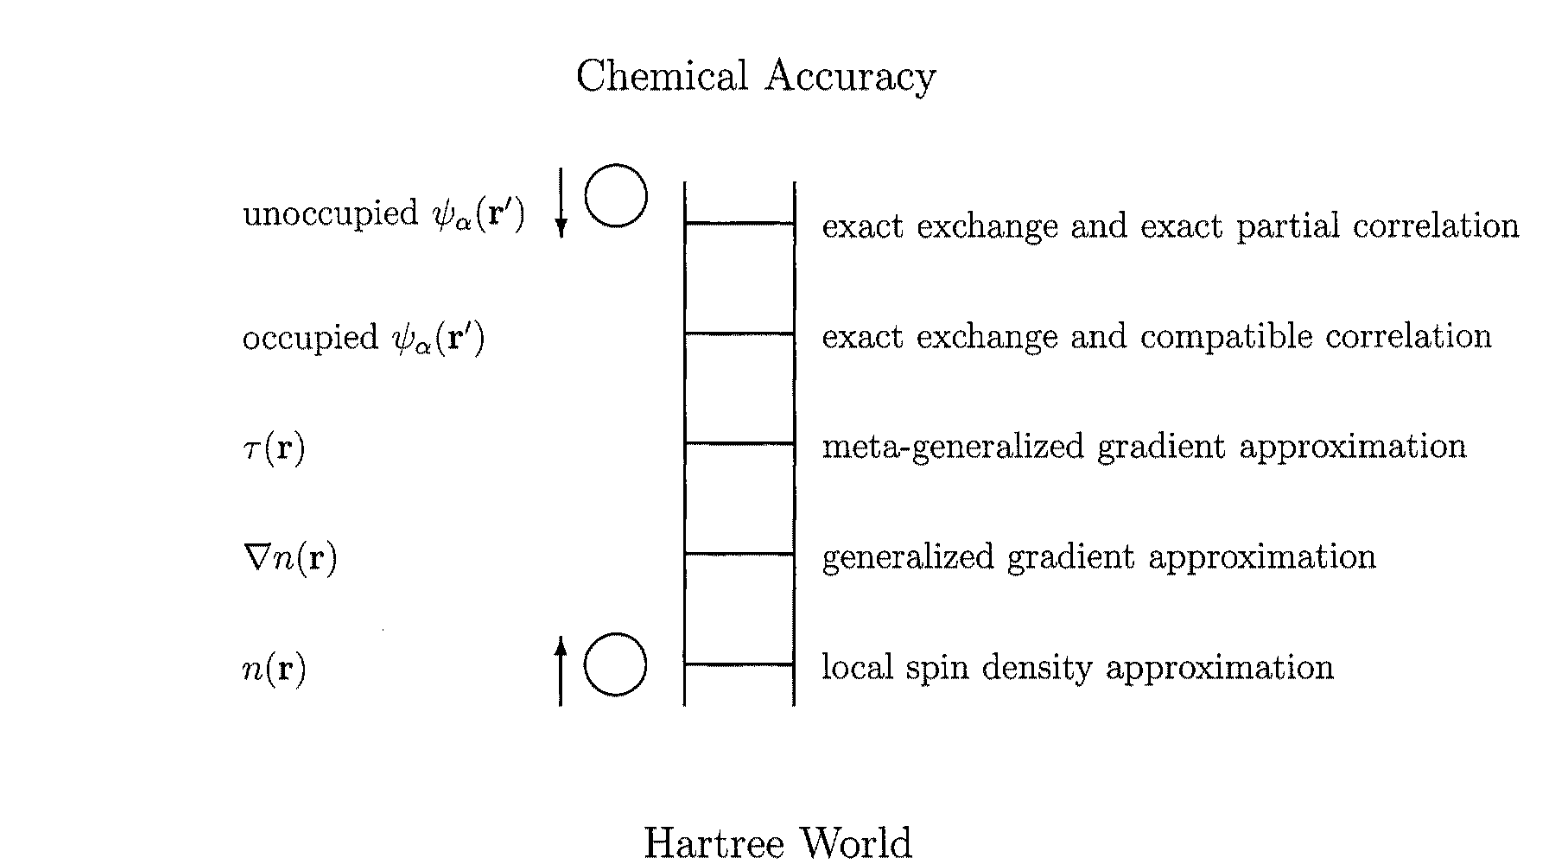
\includegraphics[width=\linewidth]{jacob-ladder.png}
    \caption[Jacob's ladder for density-functional approximations]{Jacob's ladder for density-functional approximations; figure taken from Ref.~\cite{perdew_jacobs_2001}.}
    \label{fig:jacob-ladder}
\end{figure}

Besides the quality of the approximations used, another important aspect regards which properties (and with what effort) can be predicted by either of the two approaches. While DFT is the ideal approach for the computation of ground-state densities and energies (and derived quantities), with respect to spectral properties Green's function theory is naturally more suitable, since it provides almost directly the photoemission and absorption spectra of materials. DFT instead,


\section{Koopmans spectral functionals\label{sec:intro-koopmans}}
- about the correlation discuss single-reference methods (orthonormality of the wave functions) vs real many-body functions which are never single Slater determinants

- problem of DFT (or KS-DFT) is that explicit expressions of energies and potentials in terms of the density are not known --> density-matrix, wave function, one-particle spin-orbitals or other stuff provide explicit expressions.

- Green's function natural generalization of density and density-matrix. Spectral properties are resolved in frequency space, then Green's function good because it has frequency. (see page 2 review Reining). Tracing interactions resulting at different spaces and times is very difficult with a local static object such as the density (reason for the difficulty in finding explicit expressions for observables in terms of the density). One also wants to avoid to express (expectation values of) observables in terms of the wave function, which have a trivial definition but that can be very complicate to handle because of the super complex character of the many-body wave function. This complexity is also a consequence of the fact that the many-body wave function ultimately carries more information than what we need. Therefore many observables, especially spectral properties, can be defined in terms of the Green's function.

\section{Objectives\label{sec:objectives}}

\section{Organisation of the thesis\label{sec:organization-thesis}}

